\documentclass[dvipdfmx]{jsarticle}
\usepackage{tikz}
\usetikzlibrary{calc}
\usetikzlibrary{positioning}
\usetikzlibrary{arrows.meta}

\begin{document}

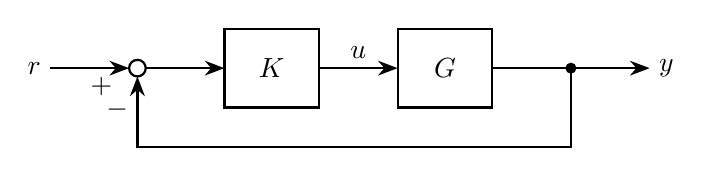
\begin{tikzpicture}
  [
  % 線と文字の間の間隔を設定
  every node/.style={outer sep=0.12cm, inner sep=0},
  % 矢印の設定
  arrow/.style={-{Stealth[length=0.25cm]}, thick},
  % ブロック
  block/.style={rectangle, draw, minimum height = 1cm,
  minimum width=1.2cm, thick, outer sep = 0},
  % 加え合わせ点
  sum/.style={thick, circle, draw, inner sep=0,
  minimum size=6pt, outer sep=0},
  % 引き出し点
  point/.style={radius=2pt}
  ]
  \node [block] (K){$K$};
  \node [block, right=1 of K] (G){$G$};
  \node [sum, left=1of K] (sum){};
  \draw[arrow] (sum) -- (K);
  \draw[arrow] (K) -- (G) node [above, pos=0.5] {$u$};
  \draw[arrow] (G.east) -- +(2, 0) node[right]{$y$};
  \draw[arrow] (sum.west)+(-1, 0) node[left]{$r$} -- (sum.west)
  node[below, xshift=-10pt]{$+$};
  \fill [point] (G.east)+(1, 0) circle coordinate (y);
  \draw [arrow] (y) -- +(0, -1) -| (sum) node[left, yshift=-15pt] {$-$};
\end{tikzpicture}

\end{document}